\documentclass{article}
\usepackage{graphicx}
\usepackage[margin=1.5cm]{geometry}
\usepackage{amsmath}

\begin{document}

\title{Thursday Reading Assessment: Unit 7, Power and Conservation of Energy}
\author{Prof. Jordan C. Hanson}

\maketitle

\section{Memory Bank}

\begin{enumerate}
\item $KE = \frac{1}{2}m v^2$ ... Definition of kinetic energy
\item $PE_G = mgh$ ... Definition of gravitational potential energy
\end{enumerate}

\section{Conservation of Energy}

\begin{enumerate}
\item A particle of mass m is hung from the ceiling by a massless string of length L, as shown in Figure \ref{fig:pend}. The particle is released from rest, when the angle between the string and the downward vertical direction is $\theta$.
\begin{figure}[ht]
\centering
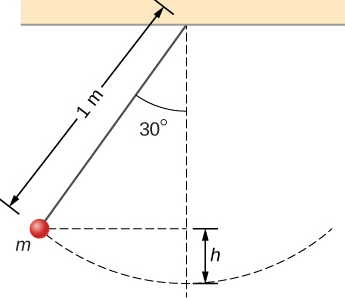
\includegraphics[width=0.4\textwidth]{pend.png}
\caption{\label{fig:pend} A particle hung from a string constitutes a simple pendulum. It is shown when released from rest, along with some distances used in analyzing the motion.}
\end{figure}
\item Show using trigonometry that the height of the pendulum is given by $h = L(1-\cos\theta)$. \\ \vspace{1cm}
\item What is the gravitational potential energy as a function of the angle $\theta$? \textit{Hint: you just found $h$, so an equation from the memory bank finishes the problem.}\\ \vspace{1cm}
\item Set the gravitational potential energy equal to the expression for kinetic energy in the memory bank.  What is its speed when it reaches the lowest point of its arc, if $\theta = 30$ deg, and $L = 1.0$ m? 
\end{enumerate}
\end{document}